\documentclass[12pt]{article}
\usepackage[a4paper, text={6.5in,9in}]{geometry}
% \usepackage[utf8]{inputenc}
\usepackage{graphicx}
\graphicspath{ {immagini/} }

% \usepackage{titling}

\usepackage{hyperref}
\hypersetup{
    colorlinks,
     citecolor=black,
     filecolor=black,
     linkcolor=black,
     urlcolor=black
 }

% \usepackage{fancyhdr}
% \pagestyle{fancy}

\usepackage{amsmath}
\usepackage{amssymb}
\usepackage{mathtools}
\usepackage{dsfont}
\usepackage{cases}
% \newcommand*{\Z}{\mathds{Z}}

\usepackage{minted, xcolor}
%\usemintedstyle{monokai}
\definecolor{bg}{HTML}{F0F0F0}
% \usepackage[defaultmono]{droidsansmono}
% \usepackage[T1]{fontenc}

% \pretitle{%
%   \begin{center}
%   \LARGE
%   \includegraphics[width=6cm]{logo-unipd}\\[\bigskipamount]
% }
% \posttitle{\end{center}}

\title{\textbf{Università di Padova \\ Formal Methods for Cyber-Physical Systems project report}}
\author{Alberto Lazari - 1216747 \\}
\date{Giugno 2022 - A.A. 2021-2022}

\renewcommand*\contentsname{Indice}

%TODO tradurre in inglese
\begin{document}
    \maketitle
    \pagebreak

    \tableofcontents
    \pagebreak

    \section{Notazione}
    \begin{description}
        \item $Post$: function which represents the set of states reachable from a given region by applying a single step of transition;
        \item $List[i]$: elemento di una lista $List$ di indice $Size(List) - i, i \in \mathbb N$.
    \end{description}

    \section{Reachability}
    \subsection{Intuitive idea}
    Given a region of initial states $Init$, a transition function $Trans$ and an invariant $Inv$, the goal of this algorithm is to decide if $Inv$ is verified in all the reachable states starting from $Init$ by applying $Trans$.

    To achieve this goal, a symbolic representation of all and only the reachable states of the system needs to be found. In this way, it is easy to check if the invariant is not verified in some of these states. An optimization can be used to avoid calculating all the states if some states that do not satisfy the invariant are found during the process.

    In order to do this, a variable $Reach$ is used to represent the reachable states of the system and it is updated iteratively.
    The basic idea is that at iteration $t$, $Reach$ represents all the states reachable from $Init$ by applying $Trans$ at most $t$ times.
    The algorithm stops when one of the following conditions is verified:
    \begin{enumerate}
        \item $Post(Reach) \subseteq Reach $: we have found all the reachable states;
        \item $Reach \cap NotInv \neq \emptyset$: we have found some reachable states in which the invariant is not verified.
    \end{enumerate}

    \textbf{TODO Disegnino}

    \subsection{Implementation}
    The implementation of the algorithm in pseudocode is the following:

    \begin{minted}[bgcolor=bg, breaklines, fontsize=\small, mathescape=true, escapeinside=||, linenos]{python}
function IsInvariantRespected(Init, Trans, Inv)
    NotInv |$\leftarrow \mathbb U\ \setminus$| Inv
    Reach |$\leftarrow$| Init
    New |$\leftarrow$| Init
    while New |$\neq \varnothing$| do
        if New |$\cap$| NotInv |$\neq \varnothing$| then
            return False
        end if
        New |$\leftarrow$| Post(New, Trans) |$\setminus$| Reach
        Reach |$\leftarrow$| Reach |$\cup$| New
    end while
    return True
end function
    \end{minted}

    For the Python implementation, it is sufficient to translate the following instructions:
    \begin{itemize}
        \item $A \leftarrow B$ becomes: \mintinline{python}{A = B}
        \item $\mathbb U\ \setminus A$ becomes: \mintinline{python}{~A}
        \item $A \neq \varnothing$ becomes: \mintinline{python}{not A.is_false()}
        \item $A \cap B \neq \varnothing$ becomes: \mintinline{python}{A.intersected(B)}
        \item $Post(A, Trans)$ becomes: \mintinline{python}{model.post(A)}
        \item $A \setminus B$ becomes: \mintinline{python}{A - B}
        \item $A \cup B$ becomes: \mintinline{python}{A + B}
    \end{itemize}

    \subsection{Proof of correctness}
    Let:
    \begin{itemize}
        \item $\mathbb U$ be the set of all the possible states of the model;
        \item $Inv \subseteq \mathbb U$ be the set of all the states that do satisfy the invariant;
        \item $NotInv \vcentcolon= \mathbb U \setminus Inv \subseteq \mathbb U$;
        \item $Reach^k$ be the set of all the states reachable in at most $k$ steps, defined as:
        $$
            \begin{cases}
                Reach^0 = Init \\
                Reach^{k + 1} = Reach^k \cup Post(Reach^k)
            \end{cases}
        $$
        \item $New^k$ be the set of all the states reachable in exactly $k$ steps, defined as:
        $$
            \begin{cases}
                New^0 = Init \\
                New^{k + 1} = Reach^{k+1} \setminus Reach^k
            \end{cases}
        $$
    \end{itemize}
    This way, $Reach^k$ and $New^k$ correspond to the values taken by the variables \texttt{Reach} and \texttt{New} at the $k$-th iteration.

    We want to prove that:
    \begin{itemize}
        % \item le definizioni date di $New^k$ e $Reach^k$ sono sound;
        \item the algorithm always terminates;
        \item $Reach^k \subseteq Inv\ \forall k$ se l'algoritmo ritorna true;
        \item if the algorithm returns true, then $Reach^k \subseteq Inv\ \forall k$;
        \item if the algorithm returns false, then $\exists k \mbox{ s.t. } Reach^k \cap NotInv \neq \varnothing$.
    \end{itemize}

    % \paragraph{Soundness of definitions}
    % \newcommand{\New}{\mathtt{New}}
    % \newcommand{\Reach}{\mathtt{Reach}}
    % Dimostriamo per induzione su $k$ che la definizione di $New$ e $Reach$ è corretta.
    % In particolare, dimostriamo che $New^k$ e $Reach^k$ corrispondono al valore delle variabili $\New^k$ e $\Reach^k$ al $k$-esimo ciclo dell'algoritmo.
    % Ovvero, vogliamo dimostrare che
    % \begin{equation}
    %     New^k = \New^k \wedge Reach^k = \Reach^k\ \forall k
    % \end{equation}

    % \subparagraph*{Caso base:}
    % $New^0 = Reach^0 = Init$ è corretto poiché corrisponde all'inizializzazione delle variabili nell'algoritmo.

    % \subparagraph*{Caso induttivo ($k+1$):}
    % Seguendo il flusso dell'algoritmo, assumendo che non sia già terminato, otteniamo:
    % \begin{equation}\label{th:sound:def_var}
    %     \begin{cases}
    %         \New^{k+1} = Post(\New^k) \setminus \Reach^k \\
    %         \Reach^{k+1} = \Reach^k \cup \New^k
    %     \end{cases}
    % \end{equation}

    % Inoltre, per definizione di $New$ e $Reach$ sappiamo che:
    % \begin{equation}\label{th:sound:def_ind}
    %     \begin{cases}
    %         Reach^{k+1} = Reach^k \cup Post(Reach^k) \\
    %         New^{k+1} = Reach^{k+1} \setminus Reach^k 
    %     \end{cases}
    % \end{equation}

    % Per ipotesi induttiva, sappiamo che:
    % \begin{equation*}
    %     \New^k = New^k \wedge \Reach^k = Reach^k
    % \end{equation*}

    % Sostituendo in (\ref{th:sound:def_var}), otteniamo
    % \begin{equation}\label{th:sound:def_var_sost}
    %     \begin{cases}
    %         \New^{k+1} = Post(New^k) \setminus Reach^k \\
    %         \Reach^{k+1} = Reach^k \cup New^k
    %     \end{cases}
    % \end{equation}

    % Per dimostrare che $\New^{k+1} = New^{k+1}\ \wedge\ \Reach^{k+1} = Reach^{k+1}$, per la (\ref{th:sound:def_ind}) e la (\ref{th:sound:def_var_sost}), è ora sufficiente dimostrare che
    % \begin{numcases}{}
    %     Reach^k \cup New^k = Reach^k \cup Post(Reach^k) \\
    %     Post(New^k) \setminus Reach^k = (Reach^k \cup New^k) \setminus Reach^k 
    % \end{numcases}

    \paragraph{Termination}
    We prove that the algorithm always terminates returning True or False.
    
    We know that $\mathbb U$ is finite, because every state is a combination of a finite and constant number of variables, which can assume a finite number of values.

    Furthermore, $\exists n$ such that:
    $$
    \begin{cases}
          New^k \subset New^{k+1} & \forall k < n \\
          New^k = New^{k+1} & \forall k \geq n
    \end{cases}
    $$

    Such $n$ must exist because the sequence $(Reach^k)_k$ is increasing (by definition of $Reach$), discrete (because it is a sequence of sets) and bounded above (because $Reach^k \subseteq \mathbb U\ \forall k$).
    
    Di conseguenza, per la definizione di $New$, avremo che $\exists n$ tale che $New^{k+1} = Reach^{k+1} \setminus Reach^k = \varnothing\ \forall k \geq n$.

    Ciò significa che in al più $n$ iterazioni, l'algoritmo esce dal ciclo principale e quando lo fa ritorna True. 

    \paragraph{Assenza di falsi positivi}
    Dimostriamo di seguito che $Reach^k \subseteq Inv\ \forall k$ se l'algoritmo ritorna true.

    È banale vedere che se l'algoritmo ritorna true, allora il ciclo while è terminato dopo $k$ iterazioni perché $New^k = \varnothing$ e in ogni iterazione precedente non si è entrati nella condizione di riga 6. Ovvero, $New^{k'} \cap NotInv = \varnothing\ \forall k' < k$.
    Inoltre, $New^k = \varnothing \subseteq Inv$.

    Di conseguenza è possibile affermare che se l'algoritmo ritorna true allora $New^{k'} \subseteq Inv\ \forall k' \leq k$.

    Procediamo ora per induzione su $k$ per dimostrare che 
    \begin{equation}\label{th:true:tesi}
        New^{k'} \subseteq Inv\ \forall k' \leq k \implies Reach^k \subseteq Inv
    \end{equation}
    
    \subparagraph*{Caso base:}
    Per $k = 0$ abbiamo $Reach^0 = Init = New^0$ per le definizioni di $Reach$ e $New$. Di conseguenza, $New^0 \subseteq Inv \implies Reach^0 \subseteq Inv$ è trivially true.

    \subparagraph*{Caso induttivo ($k+1$):}
    Vogliamo dimostrare induttivamente che
    \begin{equation}\label{th:true:ind:tesi}
        New^{k'} \subseteq Inv\ \forall k' \leq k+1 \implies Reach^{k+1} \subseteq Inv
    \end{equation}
    Possiamo assumere che $New^{k'} \subseteq Inv\ \forall k' \leq k+1$, altrimenti la parte sinistra di (\ref{th:true:ind:tesi}) è falsa e, di conseguenza, il caso induttivo è trivialmente vero.

    Vogliamo dunque dimostrare $Reach^{k+1} \subseteq Inv$ assumendo
    \begin{numcases}{}
        New^{k'} \subseteq Inv\ \forall k' \leq k+1 & \mbox{per quanto appena detto} \label{th:true:ind:ass_1} \\
        New^{k'} \subseteq Inv\ \forall k' \leq k \implies Reach^k \subseteq Inv & \mbox{per ipotesi induttiva} \label{th:true:ind:hp_ind} \\
        Reach^{k+1} = Reach^{k} \cup New^{k+1} & \mbox{per definizione di $New$} \label{th:true:ind:def_new}
    \end{numcases}

    È banale osservare che da (\ref{th:true:ind:ass_1}) seguono
    \begin{numcases}{}
        New^{k'} \subseteq Inv\ \forall k' \leq k \label{th:true:ind:hp_ind:left} \\
        New^{k+1} \subseteq Inv \label{th:true:ind:new}
    \end{numcases}

    La (\ref{th:true:ind:hp_ind}) e la (\ref{th:true:ind:hp_ind:left}) implicano
    \begin{equation}\label{th:true:ind:hp_ind:right}
        Reach^k \subseteq Inv
    \end{equation}

    Infine, dalla (\ref{th:true:ind:def_new}), la (\ref{th:true:ind:new}) e la (\ref{th:true:ind:hp_ind:right}) segue la tesi induttiva (\ref{th:true:ind:tesi}).
    
    \paragraph{Assenza di falsi negativi}
    Dimostriamo di seguito che se l'algoritmo ritorna false allora $\exists k \mbox{ s.t. } Reach^k \cap NotInv \neq \varnothing$.

    È banale vedere che l'unico caso in cui l'algoritmo ritorna false è quando all'iterazione $k$ si verifica la condizione $New^k \cap NotInv \neq \varnothing$.
    
    \section{Counterexample search}
    \subsection{Idea di base}
    Durante la ricerca degli stati raggiungibili, ad ogni iterazione viene memorizzato l'insieme $New$ in una lista.
    Se a una certa iterazione $New \cap NotInv = \varnothing$, invece di aggiungere in coda alla lista $New$ aggiungiamo $New \cap NotInv$, ovvero gli stati che non rispettano l'invariante.
    A partire da questa lista costruiamo ricorsivamente la trace degli stati che portano il sistema a non rispettare l'invariante nel seguente modo:
    \begin{itemize}
        \item \textbf{Caso base:} Se la lista ha un solo elemento E, ritorno uno stato qualsiasi in E;
        \item \textbf{Caso Induttivo:} Altrimenti, 
        \begin{enumerate}
            \item estrae dalla lista l'ultimo elemento \texttt{sym\_target};
            \item sceglie uno stato qualsiasi in \texttt{sym\_target} che chiamiamo \texttt{target};
            \item modifica il nuovo ultimo elemento della lista restringendolo in modo tale che da ogni suo elemento sia raggiungibile \texttt{target} in una iterazione;
            \item invoca ricorsivamente sulla lista modificata e concatena il risutato con \texttt{target}.
        \end{enumerate}
    \end{itemize}

    Questo algoritmo consente di poter sempre scegliere un elemento qualsiasi nella regione in coda alla lista.
    La modifica all'ultimo elemento prima della ricorsione serve a garantire il mantenimento di questa proprietà.

    \begin{figure}[H] 
        \centering
        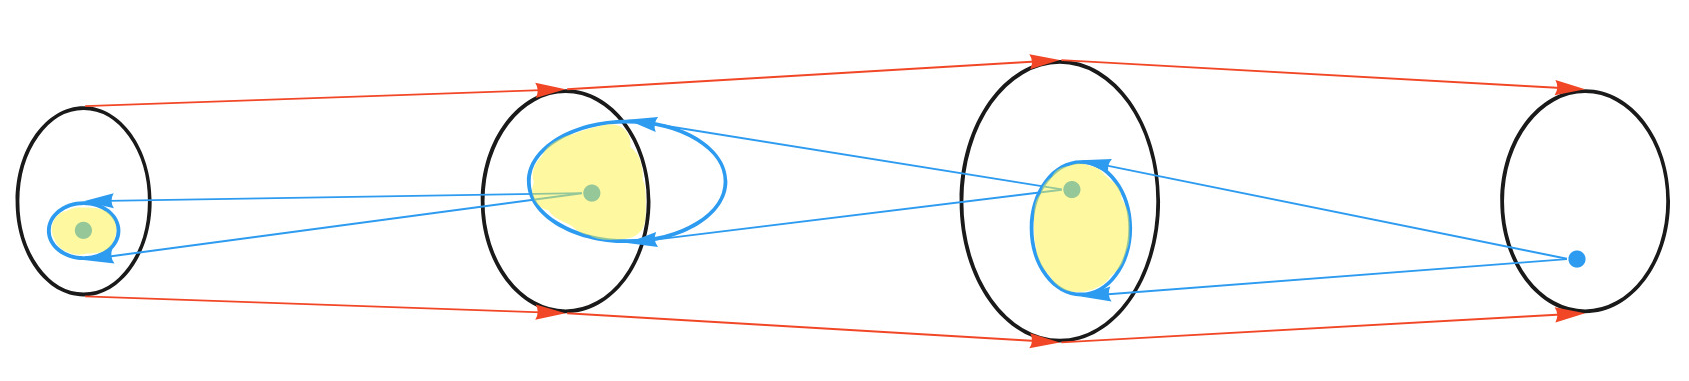
\includegraphics[width=\textwidth]{backtrace-diagram.png}
        \caption{Diagram representing the backtrace creation process.}
    \end{figure}

    \subsection{Implementazione}
    Di seguito viene riportato lo pseudocodice dell'algoritmo per creare la tracce degli stati che portano il sistema a non rispettare l'invariante:
    \begin{minted}[bgcolor=bg, breaklines, fontsize=\small, mathescape=true, escapeinside=||, linenos]{python}
function CreateTrace(SymTrace)
    if len(SymTrace) == 0 return []
    if len(SymTrace) == 1 return [PickOneState(SymTrace[0])]

    SymTarget |$\leftarrow$| SymTrace.pop()
    Target |$\leftarrow$| PickOneState(SymTarget)
    SymTrace[-1] = SymTrace[-1] |$\cap$| Pre(Target)
    Trace |$\leftarrow$| CreateTrace(SymTrace)
    Trace |$\leftarrow$| Trace + Target
    return Trace
end function
    \end{minted}
    Considerando Trace la lista di stati ottentua dalla funzione precedente, per ottenere gli input che portano il sistema da uno stato presente in Trace al successivo, basta utilizzare la funzione \mintinline{python}{GetInputsBetweenStates(State1, State2)} ed applicarla ad ogni coppia di stati adiacenti nella lista.
    
    \subsection{Dimostrazione di correttezza}
    \begin{itemize}
        \item Precondizione:
        \begin{equation}
            \begin{cases}
                i \neq j \implies SymTrace[i] \cap SymTrace[j] = \varnothing\ \forall i, j \\
                SymTrace[i] = R \wedge \exists SymTrace[i+1] \implies SymTrace[i+1] \subseteq Post(R)
            \end{cases}
        \end{equation}
        \item Postcondizione: La funzione ritorna una lista Trace di stati tali che:
        \begin{equation}
            \begin{cases}
                SymTrace[i] = R \implies Trace[i] \in R \\
                \forall i \mbox{ s.t. } 0 \leq i < SymTrace.size - 1, Trace[i+1] \in Post(\{Trace[i]\})
            \end{cases}
        \end{equation}
    \end{itemize}

    \subparagraph*{Caso base - SymTrace vuota}
    Ritorniamo una lista vuota che sottisfa trivialmente entrambe le post condizioni.

    \subparagraph*{Caso base - SymTrace con un elemento}
    SymTrace è composta da una sola regione R e ritorniamo una lista composta da uno stato qualsiasi di R.
    SymTrace[0] = R e Trace[0] $\in$ R.
    Mentre la seconda postcondizione è trivialmente vera perché Trace ha un solo elemento.

    \subparagraph*{Caso ricorsivo}
    SymTrace ha almeno due elementi.
    
    SymTrace' è il valore originale di SymTrace.

    \begin{minted}[bgcolor=bg, breaklines, fontsize=\small, mathescape=true, escapeinside=||]{python}
SymTarget |$\leftarrow$| SymTrace.pop()
Target |$\leftarrow$| PickOneState(SymTarget)
    \end{minted}

    Target $\in$ SymTrace[-1] per le proprietà della funzione PickOneState.

    SymTrace è SymTrace' privato dell'ultimo elemento
     
    \begin{minted}[bgcolor=bg, breaklines, fontsize=\small, mathescape=true, escapeinside=||]{python}
    SymTrace[-1] = SymTrace[-1] |$\cap$| Pre(Target)
    \end{minted}

    Target $\in$ Post(\{s\}) $\forall$ s $\in$ SymTrace[-1]

    La precondizione della chiamata ricorsiva è rispettata perché:
    \begin{itemize}
        \item se SymTrace' è una lista di regioni disgiunte allora anche Symtrace[0:-1] = SymTrace'[0:-2] è una lista di regioni disgiunte;
        inoltre, SymTrace[-1] $\subseteq$ SymTrace'[-2] implica che SymTrace[-1] è disgiunto da tutti gli altri elementi di SymTrace;
        \item Data la precondizione e dato che $\forall i \mbox{ t.c. } 0 \leq i < SymTrace.size - 1 : SymTrace[i] = Symtrace'[i]\ e\ SymTrace[-1] \subseteq SymTrace'[-2] $, allora
        \begin{equation}
            \forall i \mbox{ s.t. } 1 \leq i < SymTrace.size, \forall e \in SymTrace[i],  e \in Post(SymTrace[i-1])
        \end{equation}
    \end{itemize}

    \begin{minted}[bgcolor=bg, breaklines, fontsize=\small, mathescape=true, escapeinside=||]{python}
 Trace |$\leftarrow$| CreateTrace(SymTrace)
    \end{minted}

    quindi Trace' = CreateTrace(SymTrace) rispetta la postcondizione di CreateTrace.
    
    \begin{minted}[bgcolor=bg, breaklines, fontsize=\small, mathescape=true, escapeinside=||]{python}
    Trace |$\leftarrow$| Trace + Target
    \end{minted}

    La Postcondizione è rispettata se:
    \begin{numcases}{}
        SymTrace[i] = R \implies Trace[i] \in R; \label{th:trace:ric:dim-post:1} \\
        \forall i \mbox{ s.t. } 0 \leq i < SymTrace.size - 1, Trace[i+1] \in Post(\{Trace[i]\}). \label{th:trace:ric:dim-post:2}
    \end{numcases}

    (\ref{th:trace:ric:dim-post:1}) è rispettata:
    \begin{itemize}
        \item per tutti gli elementi tranne l'ultimo, a seguito della postcondizione ricorsiva;
        \item per l'ultimo elemento di Trace = Target $\in$ SymTrace[-1], perché ottenuto tramite PickOneState(SymTrace[-1]).
    \end{itemize}

    (\ref{th:trace:ric:dim-post:1}) è rispettata:
    \begin{itemize}
        \item $\forall i \mbox{ s.t. } 0 \leq i < SymTrace.size - 2$ a seguito della postcondizione ricorsiva;
        \item Trace[-1] = target $\in Post(\{Trace[-2]\})$, perché target è ottenuto tramite PickOneState(SymTrace[-1]) e SymTrace[-1] $\subseteq$ Post(SymTrace[-2]).
    \end{itemize}
\end{document}
